\chapter{Программная реализация анализатора и инфраструктуры}

Данная реализация анализатора является первичной и её главная задача это иллюстрация работоспособности метода анализа.
Поэтому данный анализатор включает дополнительную инфраструктуру, не рассматриваемую в методе. Такие компоненты
анализатора будут отмечены соответствующим примечанием в тексте.

\section{Общая архитектура}

\subsection{Составляющие анализатора}

Исходя из раздела \ref{sec:architecture} анализатор, реализующий описываемый метод мультиязыкового анализа будет включать в себя следующие
компоненты:
\begin{enumerate}[1)]
    \item провайдер конфигурации и кода,
    \item мультиязыковой транслятор,
    \item решатель ограничений,
    \item адаптер для конкретного инструментального средства (в данном случае LSP сервера).
\end{enumerate}

Более подробный состав анализатора представлен на диаграмме компонентов на рисунке \ref{fig:components}.

\begin{figure}[H]
    \centering
    \resizebox{0.9\linewidth}{!}{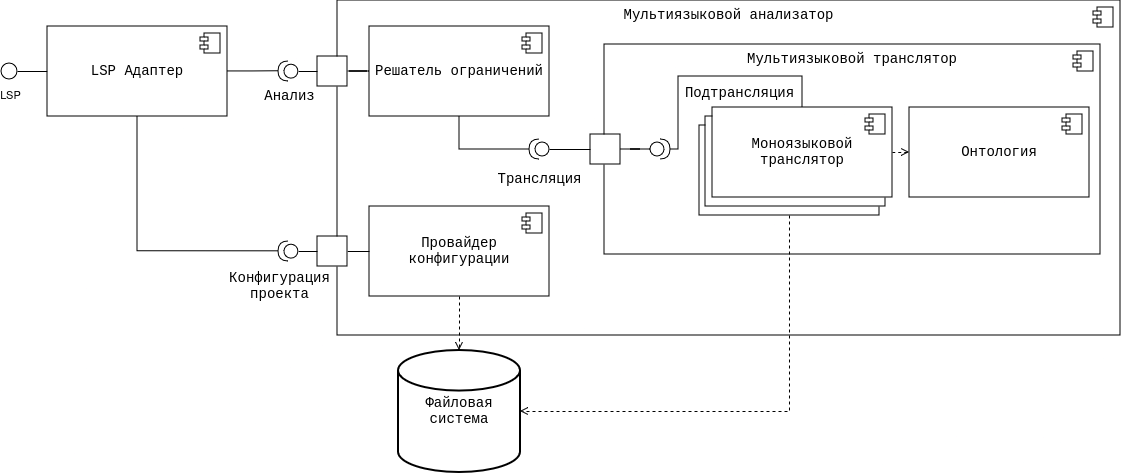
\includegraphics[height=0.85\textheight]{inc/img/components}}
    \caption{Диаграмма компонентов анализатора}
    \label{fig:components}
\end{figure}

Также, порядок запросов к анализатору и вызовы соответствующих процедур приведены на диаграмме деятельности
на рисунке \ref{fig:sequence}.

\begin{figure}[H]
    \centering
    \resizebox{\linewidth}{!}{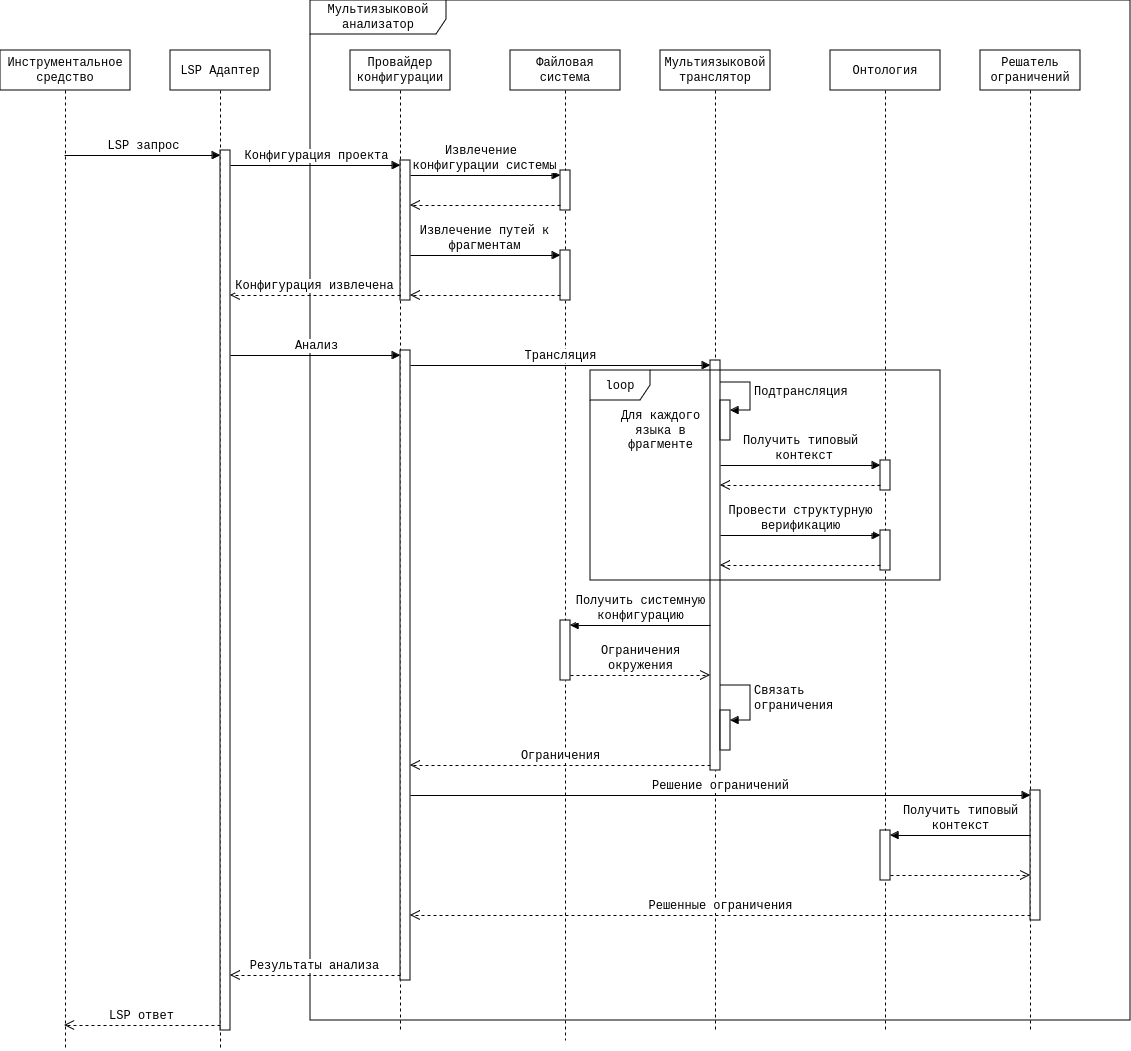
\includegraphics[height=0.85\textheight]{inc/img/sequence}}
    \caption{Диаграмма деятельности анализатора}
    \label{fig:sequence}
\end{figure}

Стоит сразу уточнить несколько деталей относительно представленных диаграмм:
\begin{enumerate}[1)]
    \item диаграммы представлены на русском языке, на довольно высоком уровне -- это сделано с целью упрощения
    понимания компонентов анализатора,
    \item на диаграммах не представленно кеширование результатов анализа,
    \item на диаграмме деятельности представлен самый благоприятный сценарий, без возникновения ошибок -- в случае ошибок
    используется стандартный механизм возврата ошибок JSON-RPC \cite{JSON-RPC}.
\end{enumerate}

\subsection{Протоколы взаимодействия}

Приведенные на рисунке \ref{fig:components} интерфейсы компонентов являются протоколами взаимодействия.
Каждый компонент в сущности представляет собой отдельное приложение, поэтому такие протоколы описывают в первую очередь межпроцессное взаимодействие.
Такой подход к структуре анализатора был сделан по следующим причинам:
\begin{enumerate}[1)]
    \item увеличение гибкости анализатора для расширения (в первую очередь в части количества моноязыковых трансляторов),
    \item поддержка использования многозадачности системы для одновременного анализа множества фрагментов,
    \item поддержка различных языков и технологий реализации компонентов.
\end{enumerate}

Стоит обратить внимание на заключительный пункт -- в отличие от некоторых мультиязыковых анализаторов, рассмотренных в разделе \ref{sec:num2},
подход с использованием обобщенной модели и общего протокола позволяет абстрагироваться от деталей реализации конкретного транслятора.
Это может быть полезно к примеру в том случае, если для анализируемого языка уже существует инфраструктура для анализа и она на другом языке
(чаще всего на нем самом). 

К примеру, можно привести инфраструктуру LLVM и в частности Clang для анализа C++ --
в проекте существует множество различных инструментов анализа C++, от построения AST и CFG до проведения различных оптимизаций.
Разработчик моноязыкового транслятора может использовать эту инфраструктуру свободно, в его обязанность входит лишь
сопровождение результатов анализа в опредленной протоколом форме.
Этот факт, в свою очередь, в целом позволяет использовать различные техники статического анализа (межпроцедурный анализ, построение DFG,
абстрактная интерпретация) что повышает гибкость моноязыковых трансляторов без изменения всего анализатора. 

Каждый из используемых протоколов базируется на механизме JSON-RPC. Это позволяет учесть стандартные
сценарии возникновения ошибок при передаче данных или во время анализа, а также устанавливает
совместимость с популярными инструментами (в первую очередь LSP). Описание всех протоколов
в качестве общего протокола приведено в приложении \ref{cha:appendix1}.
В качестве языка описания используется TypeScript так как
его типовые определения имеют достаточно высокую выразительность и его типы напрямую могут быть отражены в типы JSON.

\subsection{Реализация онтологии}

Как сказано в подразделе \ref{ssec:ontology}, онтология в данной работе является собирательным названием
механизмов поддержания консистентности.

Программная реализация таких механизмов была сделана при помощи использования отдельной виртуальной машины
в мультиязыковом трансляторе \cite{goja}. Такая машина является встраиваемым в приложение решением и
направлена на исполнение кода JavaScript.

Подход по встраиванию виртуальной машины был избран по следующим причинам:
\begin{itemize}
    \item скрипты JavaScript являются отдельной точкой расширения мультиязыкового анализатора и не затрагивают его компоненты, что повышает
    модульность,
    \item JavaScript является самым удобным средством для работы с JSON, так как является его суперсетом,
    \item использование полноценного языка программирования в отличие от языка описания данных позволяет
    без излишнего усложнения расширять функциональность онтологии.
\end{itemize}

\section{Провайдер конфигурации и кода}

В задачи провайдера конфигурации входит:
\begin{itemize}
    \item создание <<слепка>> файловой системы проекта в виде списка дерева каталогов и файлов,
    \item создание базы данных окружения системы (переменные окружения, версии системных утилит и библиотек).
\end{itemize}

Ключевой особенностью провайдера является формат результирующих данных -- после исполнения описанных задач, провайдер
должен предоставить информацию в формате ограничений. Таким образом, информация об операционном окружении
естественным образом включается в общую структуру графа областей. Это позволяет реализовывать разрешение имен
не только на уровне языков, но и на уровне окружения, что может быть полезно в случае языков командной строки
или языков сборки -- в них идентификаторы команд часто используются из содержимого файловой системы.

Вопрос извлечения кода может быть рассмотрен в виде отдельного компонента анализатора (и ранее он так и
рассматривался), но для упрощения архитектуры решено было совместить его с провайдером конфигурации.
Задачей компонента извлечения является получение путей к файлам проекта, которые нужно проанализировать.
В простейшем случае этого можно достичь путем рекурсивного обхода директорий с выборкой файлов с определенным
расширением. Именно такой подход был избран для текущей реализации анализатора. Однако, выборка
файлов может быть достаточно сложным процессом по ряду причин, описанных в подразделе \ref{ssec:selection}.

\section{Мультиязыковой транслятор}

В общем случае, использование отдельного транслятора, реализованного для конкретного языка отдельно
от остальных трансляторов является неразумным решением, так как происходит потеря информации о переплетении
фрагментов кода на разных языках в рамках одного большого фрагмента. Поэтому, логичным выглядит реализация
<<мультиязыкового>> транслятора, который будет использовать различные монотрансляторы. Но чтобы такой
транслятор работал корректно, нужен механизм 
распознавания определенного языка программирования по входной строке. Таким образом,
трансляция определенного языка будет вовлекать распознавание фрагментов языков, описанных через различные фрагменты кода.
После распознавания такие фрагменты будут направлены соответствующим трансляторам.

Таким образом, общий алгоритм трансляции выглядит следующим образом:
\begin{enumerate}[1)]
    \item на вход мультиязыковому транслятору поступает фрагмент кода,
    \item транслятор использует инструмент распознавания для подбора соответствующего монотранслятора и отправляет ему этот фрагмент,
    \item на вход транслятору поступает фрагмент кода на определенном языке,
    \item транслятор использует любые подходящие средства для анализа и трансляции данного кода
    (AST, CFG, абстрактная интерпретация и т.д.),
    \item если транслятор обнаруживает строковый литерал он может отправить его на распознавание мультиязыковому транслятору, который
    позволит определить язык избранного фрагмента и в дальнейшем направит этот фрагмент другому транслятору,
    \item все трансляторы всех языков выводят ограничения в общий буфер мультиязыкового транслятора, для последующего разрешения.
\end{enumerate}

В качестве инструмента распознавания можно использовать инструменты машинного обучения для классификации. К примеру,
на данный момент существуют довольно мощные инструменты по распознаванию кода основанные на нейронных сетях \cite{guesslang}.
Однако, в данном анализаторе был использован более простой подход: путем отправки фрагмента всем имеющимся
трансляторам можно сразу получить все необходимые данные -- в таком случае сообщение об ошибке придет от всех трансляторов, кроме одного.
Результаты именно этого транслятора являются верными.

Результаты трансляции различных монотрансляторов объединяются в контексте системного окружения. Объединение не
вовлекает решения ограничений, происходит простое связывание узлов графа областей и переменных типовых ограничений.
Следует заметить, что в текущей версии
анализатора не реализован инкрементальный подход к извлечению конфигурации и трансляции, однако концептуальных
препятствий к этому нет и такие процессы могут быть организованы инкрементально для повышения быстродействия.

\section{Решатель ограничений} \label{sec:solver}

Алгоритм решения ограничений подробно описан в \cite{scope-graphs-static-analysis} и в данной работе не изменяется.
Дополнительные ограничения, вводимые в данной работе служат лишь дополнительным источником информации для
инструментального средства и не задействованы в алгоритме разрешения имен.

Оригинальная статья описывает сценарий, при котором одной ссылке может сопоставиться несколько объявлений.
В таком случае описывается процесс деления вычисления на ветви, по ветви на каждое возможное определение.
Так как такая недетерминированность сильно замедляет вычисление, в данном анализаторе было принято решение
принебречь полнотой анализа и брать первое совпадающее определение.

В результате работы алгоритма решения ограничений формируется типовый контекст $\psi$ и известный граф областей
$G$. С точки зрения решателя это означает, что можно сформировать \textit{решенные ограничения} -- ограничения,
в которых не присутствуют неизвестные переменные. Такие ограничения можно называть фактами о проекте.

Стоит заметить, что в случае неполного решения ограничений (алгоритм заходит в тупик при наличии необработанных ограничений),
результат решения всё еще актуален и его можно использовать для дальнейшей отправки в инструментальное средство.
К сожалению, авторами статьи не было формально доказано соответствие нерешенных ограничений действительно присутствующим
ошибкам в коде, поэтому часть нерешенных ограничений не может быть использована в качестве источника информации об ошибках.

Как и в оригинальной статье, инкрементальная реализация алгоритма не была рассмотрена по причине высокой сложности
и некоторых технических вопросов в оригинальном описании алгоритма. Однако, как и в случае с трансляцией,
концептуальных препятствий к созданию инкрементального алгоритма решения ограничений нет.

\section{Адаптер инструментального средства}

Адаптер представляет собой сервер LSP, умеющий исполнять определенные сценарии LSP \cite{lsp-usecases}.
Сервер написан на TypeScript в первую очередь по причине присутствия нативного API для
работы с методами LSP и соответствующими структурами данных.

Конфигурация мультиязыкового анализатора создана с учетом stateless реализации, т.е. сам анализатор не хранит
состояние вычислений после определенных этапов. Вместо этого, было решено вынести этот слой управления состоянием
в инструментальное средство, в данном случае сервер LSP. Такой подход позволяет упростить анализатор и сделать его более гибким.

Еще одной важной особенностью является принцип работы сервера -- в отличие от многих существующих серверов LSP для
определенных языков, такой сервер не взаимодействует с файлами проекта напрямую. Единственная информация о проекте
которая ему известна это решенные ограничения, т.е. факты об областях, идентификаторах и типах. С каждым ограничением
связывается определенное местоположение -- откуда такое ограничение было получено. Такая конструкция подзволяет
облеспечить сервер всей необходимой информацией по межъязыковым зависимостям.

В связи с этим появляется несколько особенностей, которые делают применение мультиязыкового анализатора в сервере LSP
специфическим:
\begin{itemize}
    \item инкрементальный анализ является нелинейным,
    \item сообщения об ошибках не могут связаны с процессом решения ограничений.
\end{itemize}

В оригинальной статье \cite{scope-graphs-static-analysis} при разработке алгоритма разрешения имен, авторами
учитывается очень важное свойство графов областей -- нелинейность при разрешении имен. Используя пример авторов:
допустим, существует граф $G$ в котором ссылка $r_i$ в области $S$ разрешается в объявление $d_i$ в родительской области $S'$.
Тогда, в большем графе $G'$, в котором объявление $d_j$ находится уже в самой области $S$, ссылка $r_i$ неизбежно
будет разрешена именно в это объявление, а старое объявление из $S'$ будет затенено.
Таким образом, при увеличении графа, предыдущие результаты решения графа могут оказаться неверными, что
может обязывать в необходимости запуска решателя еще один раз.

Как было сказано в \ref{sec:solver}, нерешенные ограничения не могут быть использованы напрямую как источник
ошибок, по крайней мере это не было доказано. Именно поэтому список ограничений был дополнен \textit{ограничениями консистентности},
которые позволяют инструментальному средству определить ошибочную ситуацию и составить соответствующий отчет.

Стоит заметить, что гибкость мультиязыкового анализатора позволяет учесть обе вышеперечисленные особенности,
если имеется возможность вовлечения эвристик о предметной области анализа -- в первую очередь о языках и
их возможных связях. Например, запуск решателя на всех ограничениях после изменения или дополнения некоторых файлов не всегда
необходим, так как такие файлы могут не изменять межъязыковые связи вовсе. Добавление таких эвристик
часто присутствует в таких инструментах как LSP сервер и мультиязыковой анализ в данном случае не становится исключением.

Для интеграции полученного сервера в инструментальное средство решено было использовать Visual Studio Code и соответствующий
API. Для данной задачи было разработано небольшое расширение и предоставлены команды для работы с LSP сервером
через UI. Такие команды описаны в таблице \ref{lsp-methods}. Стоит заметить, что локальная конфигурация команд и кеширование
не описываются, так как это аспект реализации конкретного расширения для IDE.

\begin{table}[H]
    \caption{Команды для работы с мультиязыковым сервером LSP из Visual Studio Code}
    \begin{tabular}{|p{4cm}|p{4cm}|p{7cm}|}
    \hline Команда & Используемая информация & Описание команды \\ 
    \hline \texttt{crossy/configure} & Путь к проекту & Сбор информации об операционном окружении проекта \\
    \hline \texttt{crossy/translate} & Путь к онтологии & Трансляция кода проекта с сохранением полученных ограничений \\
    \hline \texttt{crossy/solve} & Путь к онтологии & Решение ограничений и сохранение полученной подстановки \\
    \hline \texttt{crossy/analyze} & Путь к онтологии & Выполнение трансляции и решения ограничений с применением полученной подстановки \\
    \hline \texttt{crossy/reset} & -- & Удаление сохраненного кеша \\
    \hline
    \end{tabular}\label{lsp-methods}
\end{table}